\chapter{有限体积法}
有限体积法的基本思想是:把计算域分成许多互不重叠的控制体或控制容积,然后在每一个
控制容积上将微分方程进行积分,用表示网格节点之间的分段分布关系来计算所要求的积分
,进而得到一个仅包含网格节点处$\phi$值表示的离散化线性方程组。

\section{稳态传导方程的有限体积法}
以某一运动要素$\phi$的一维稳态传导问题为例:
\begin{equation}
  \frac{\mathrm{d}}{\mathrm{d} x}(\Gamma \frac{\mathrm{d} \phi}{\mathrm{d} x}) +
  S = 0
\end{equation}
其中,$\Gamma$为传导系数,$S$为源项。在边界点上$\phi$的值给定。这类问题的一个例
子就是第三章讨论的一根金属棒上一维热传导问题。

\subsection{步骤一:网格生成}
有限体积法的第一步是将计算区域划分为互不重叠的离散控制体。在A和B之间均匀的布置一
系列的节点。每个控制体的边界位于相邻节点的中线处。这样,每个节点都被一个控制体或
控制单元所包围。在计算域边界处设置控制体是比较常见的做法,这样可以让控制体的边界
与物理边界重叠。
\begin{figure}[h]
  \centering
  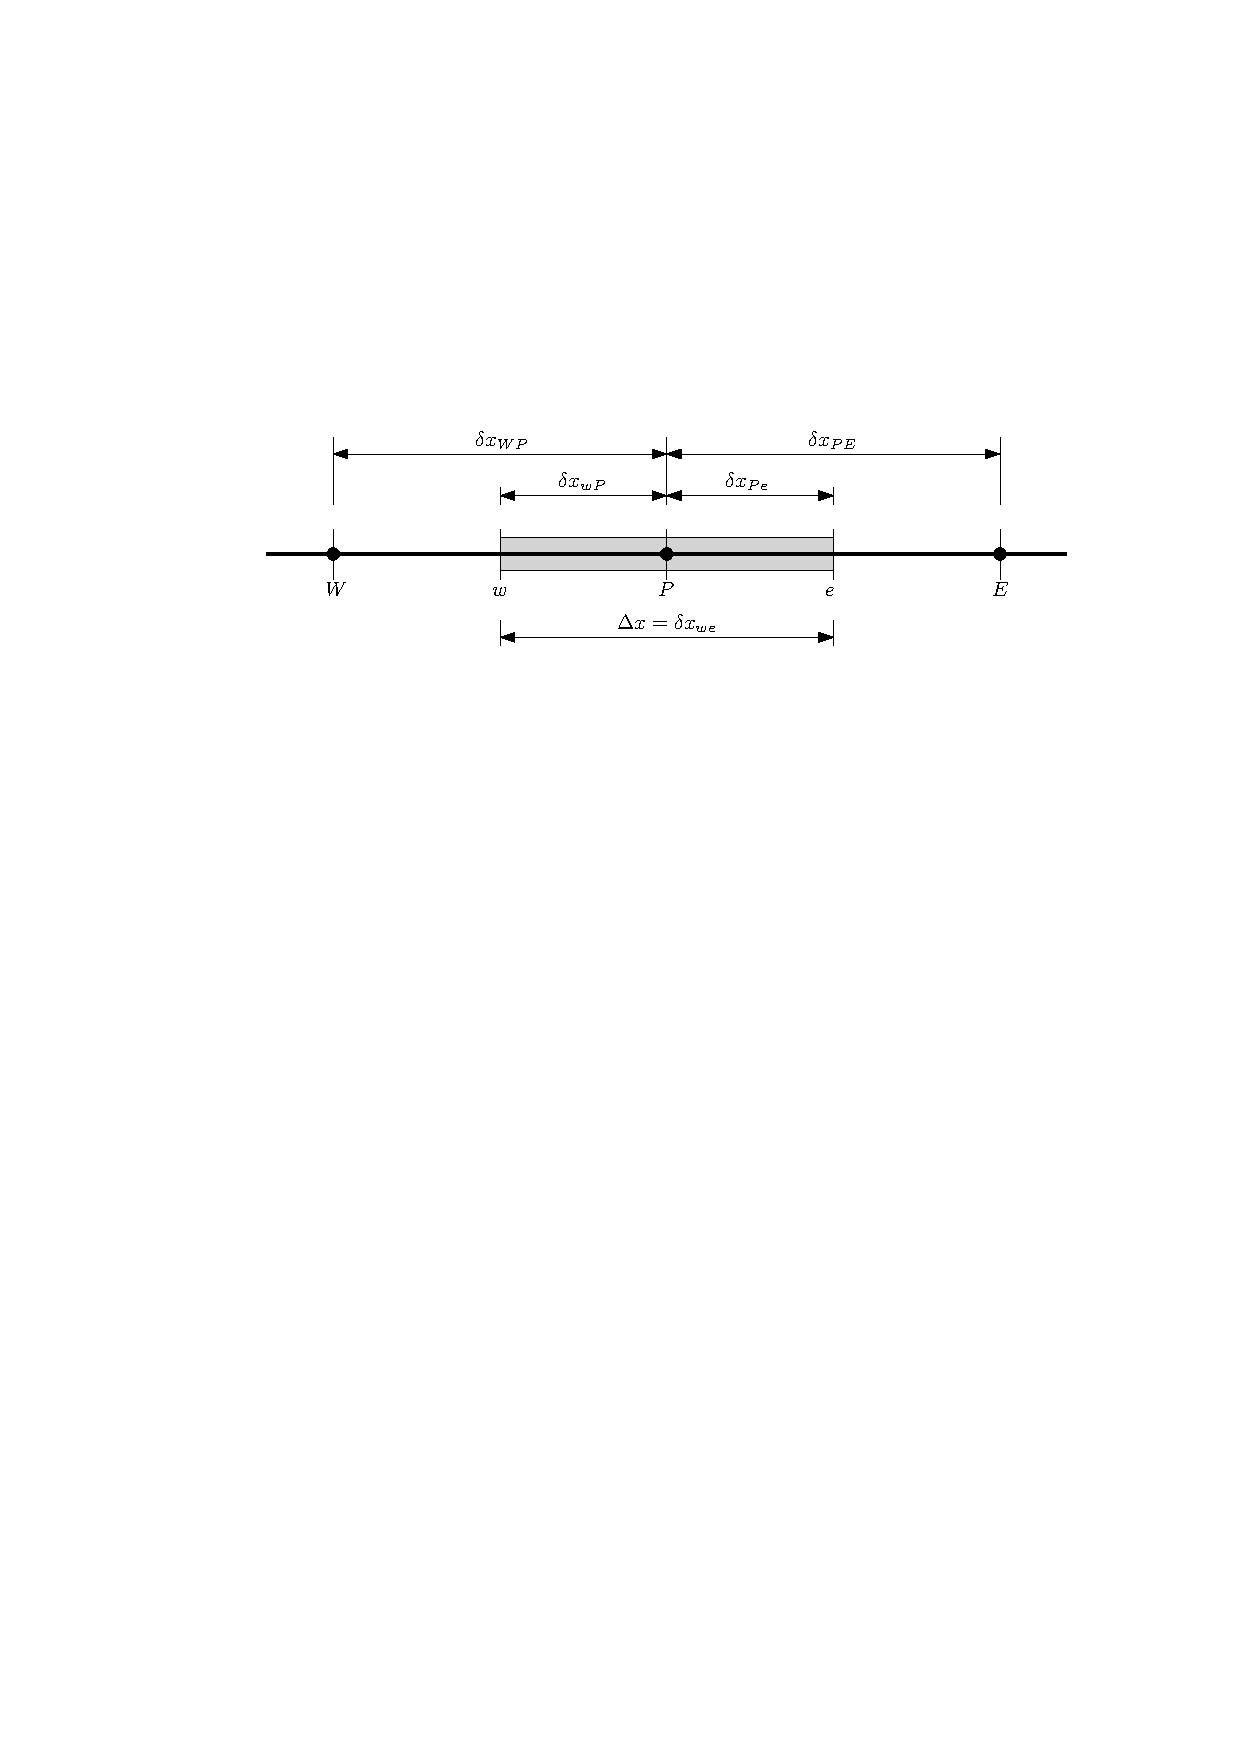
\includegraphics{FVmGridNotation.pdf}
  \caption{有限体积法一维网格系统}
  \label{FgFV_grid_notation}
\end{figure}

首先,我们建立有限体积法网格系统的符号系统。图\ref{FgFV_grid_notation}给出了计算域中网格系统的示意
图。图中$P$为网格系统中的任意节点,与它相邻的西侧和东侧节点分别为$W$和$E$。节点
$P$所在控制体(灰色区域)西边的边界面为$w$,东边的边界面为$e$。$W$节点与$P$节点的距离为
$\delta x_{WP}$,$P$节点与$E$节点的距离为$\delta x_{PE}$。控制体边界面$w$到$P$节
点的距离为$\delta x_{wP}$,$P$节点到边界面$e$的距离为$\delta x_{Pe}$,边界面$w$
到边界面$e$的距离为$\delta x_{we}$。


\subsection{步骤二:离散}
有限体积法的关键步骤是在控制体上对控制方程积分来得到控制体节点$P$上的离散方程。
对上面建立的网格系统,
\begin{equation}
  \int_{\Delta V}\!
  \frac{\mathrm{d} }{\mathrm{d} x}
  \left(
    \Gamma \frac{\mathrm{d} \phi}{\mathrm{d} x}
  \right)
  \mathrm{d}V
  +
  \int_{\Delta V}\!
  S
  \mathrm{d}V
  =
  \left(
    \Gamma A\frac{\mathrm{d} \phi}{\mathrm{d} x}
  \right)_{e}
  -
  \left(
    \Gamma A\frac{\mathrm{d} \phi}{\mathrm{d} x}
  \right)_{w}
  +
  \overline{S}\Delta V
  =
  0
  \label{EqFV_Diffusion_Discretisation}
\end{equation}
式中,$A$为控制体边界面的面积,$\Delta V$为控制体体积,$\overline{S}$为控制体上
$S$的平均值。有限体积法的一个非常吸引人的特性是离散方程具有明确的物理意义。式
\eqref{EqFV_Diffusion_Discretisation}表明:流出东边交界面的$\phi$的扩散通量减去流
入西边交界面的$\phi$的扩散通量等于$\phi$的减少量。

为了推导出可用的离散方程,式\eqref{EqFV_Diffusion_Discretisation}中控制体交界面上的
$\Gamma$和梯度$\mathrm{d}\phi/\mathrm{d}x$必须要先求得。
\begin{subequations}
  \begin{align}
  \Gamma_{w} 
  &=
  \frac{\Gamma_{W}+\Gamma_{P}}{2}
  \\
  \Gamma_{e} 
  &=
  \frac{\Gamma_{P}+\Gamma_{E}}{2}
  \end{align}
\end{subequations}
\begin{subequations}
  \begin{align}
  &\left(
    \Gamma A\frac{\mathrm{d} \phi}{\mathrm{d} x}
  \right)_{e}
  =
  \Gamma_{e}A_{e}
  \left(
    \frac{\phi_{E}-\phi_{P}}{\delta x_{PE}}
  \right)
    \\
  &\left(
    \Gamma A\frac{\mathrm{d} \phi}{\mathrm{d} x}
  \right)_{w}
  =
  \Gamma_{w}A_{w}
  \left(
    \frac{\phi_{P}-\phi_{W}}{\delta x_{WP}}
  \right)
  \end{align}
\end{subequations}
\begin{equation}
  \overline{S}\Delta V = S_{u} + S_{P}\phi_{P}
\end{equation}
\begin{equation}
  \Gamma_{e}A_{e}
  \left(
    \frac{\phi_{E}-\phi_{P}}{\delta x_{PE}}
  \right)
  -
  \Gamma_{w}A_{w}
  \left(
    \frac{\phi_{P}-\phi_{W}}{\delta x_{WP}}
  \right)
  +
  (S_{u} + S_{P}\phi_{P})
  =
  0
\end{equation}
\begin{equation}
  \left(
    \frac{\Gamma}{\delta x_{PE}}A_{e}
    +
    \frac{\Gamma}{\delta x_{WP}}A_{w}
    -
    S_{p}
  \right)
  \phi_{P}
  =
  \left(
    \frac{\Gamma_{w}}{\delta x_{WP}}A_{w}
  \right)\phi_{W}
  +
  \left(
    \frac{\Gamma_{e}}{\delta x_{PE}}A_{e}
  \right)\phi_{E}
  +
  S_{u}
\end{equation}
\begin{equation}
  a_{P}\phi_{P} = a_{W}\phi_{W} + a_{E}\phi_{E}+S_{u}
  \label{EqFV_1dsd_fvm}
\end{equation}
其中
\begin{table}[H]
  \begin{center}
  %\caption{雅可比迭代结果}
  \label{TbFV_diffusion_coefficient}
  \begin{tabular}{|c|c|c|}
    \hline
    $a_{W}$ & $a_{E}$ & $a_{P}$
    \\
    \hline
    \makecell*[c]{
    $\displaystyle \frac{\Gamma_{w}}{\delta x_{WP}}A_{w}$
  }
            &
    $\displaystyle \frac{\Gamma_{e}}{\delta x_{PE}}A_{e}$
            &
    $a_{W} + a_{E} - S_{P}$
    \\
    \hline
  \end{tabular}
  \end{center}
\end{table}

\subsection{步骤三、求解}
式\eqref{EqFV_1dsd_fvm}必须在所有控制体的节点上都列出才能求解。对于毗邻计算域边
界的控制体,式\eqref{EqFV_1dsd_fvm}必须经过适当修正以包含边界条件。最后形成的线
性代数方程组可以通过上一章的求解方法来进行求解得到$\phi$的分布。

\section{一维稳态热传导问题求解}
\subsection{无源一维稳态热传导问题}
\begin{figure}[h]
  \centering
  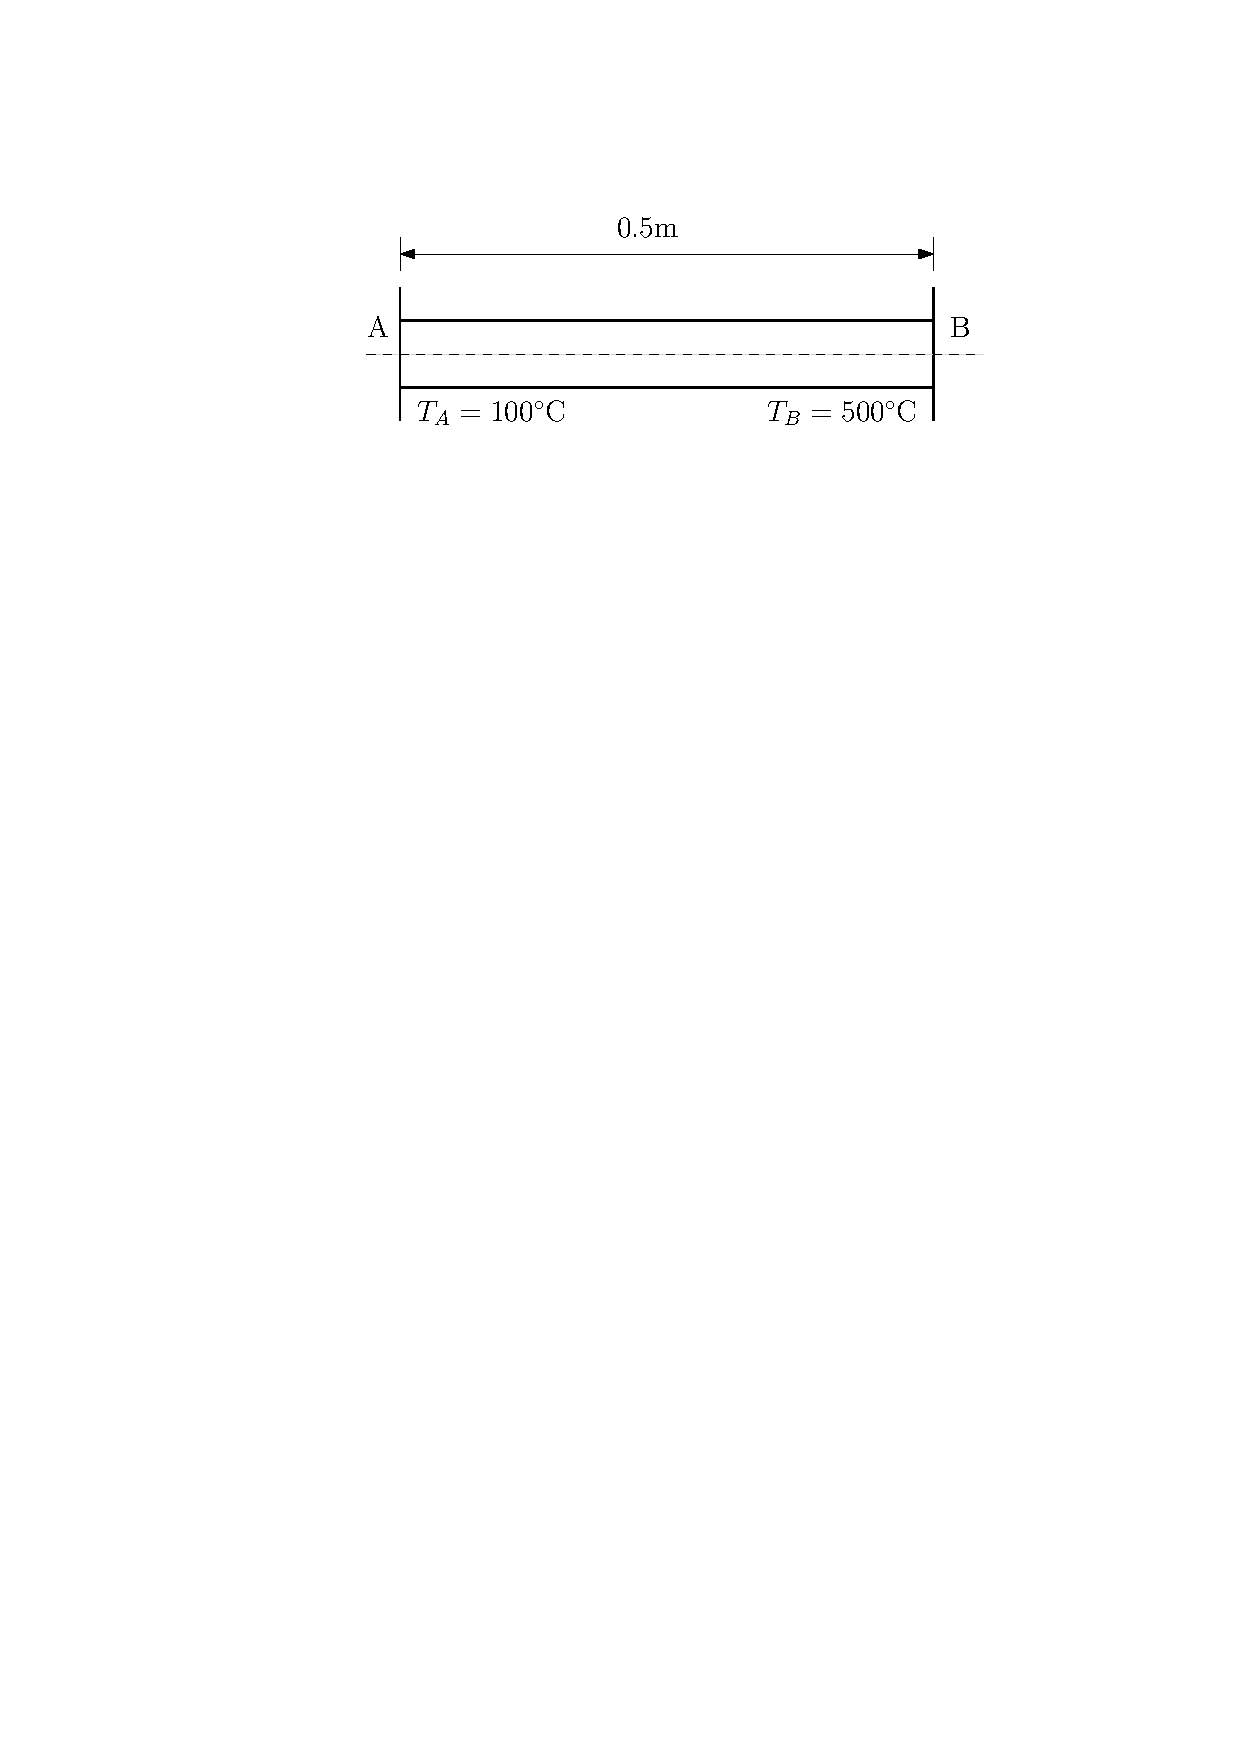
\includegraphics{FVmEx1.pdf}
  \caption{一维金属棒热传导问题}
  \label{FgFV_ex1}
\end{figure}

如图\ref{FgFV_ex1}考虑一根等直径的绝热金属棒,两端温度分布保持在
$100^{\circ}\mathrm{C}$和$500^{\circ}\mathrm{C}$。该金属棒的导热系数为常数$k$,
截面面积为$A$。该问题的控制方程为:
\begin{equation}
\frac{\mathrm{d} }{\mathrm{d} x}
\left(
k\frac{\mathrm{d} T}{\mathrm{d} x}
\right)
=
0
\label{EqFV_1dsd_ex1_gov}
\end{equation}

首先将该金属棒分成5个体积相等的控制体,如图\ref{FgFV_ex1_grid}所示。网格间
距$\delta x=0.1\mathrm{m}$。整个网格系统包括5个节点。
\begin{figure}[h]
  \centering
  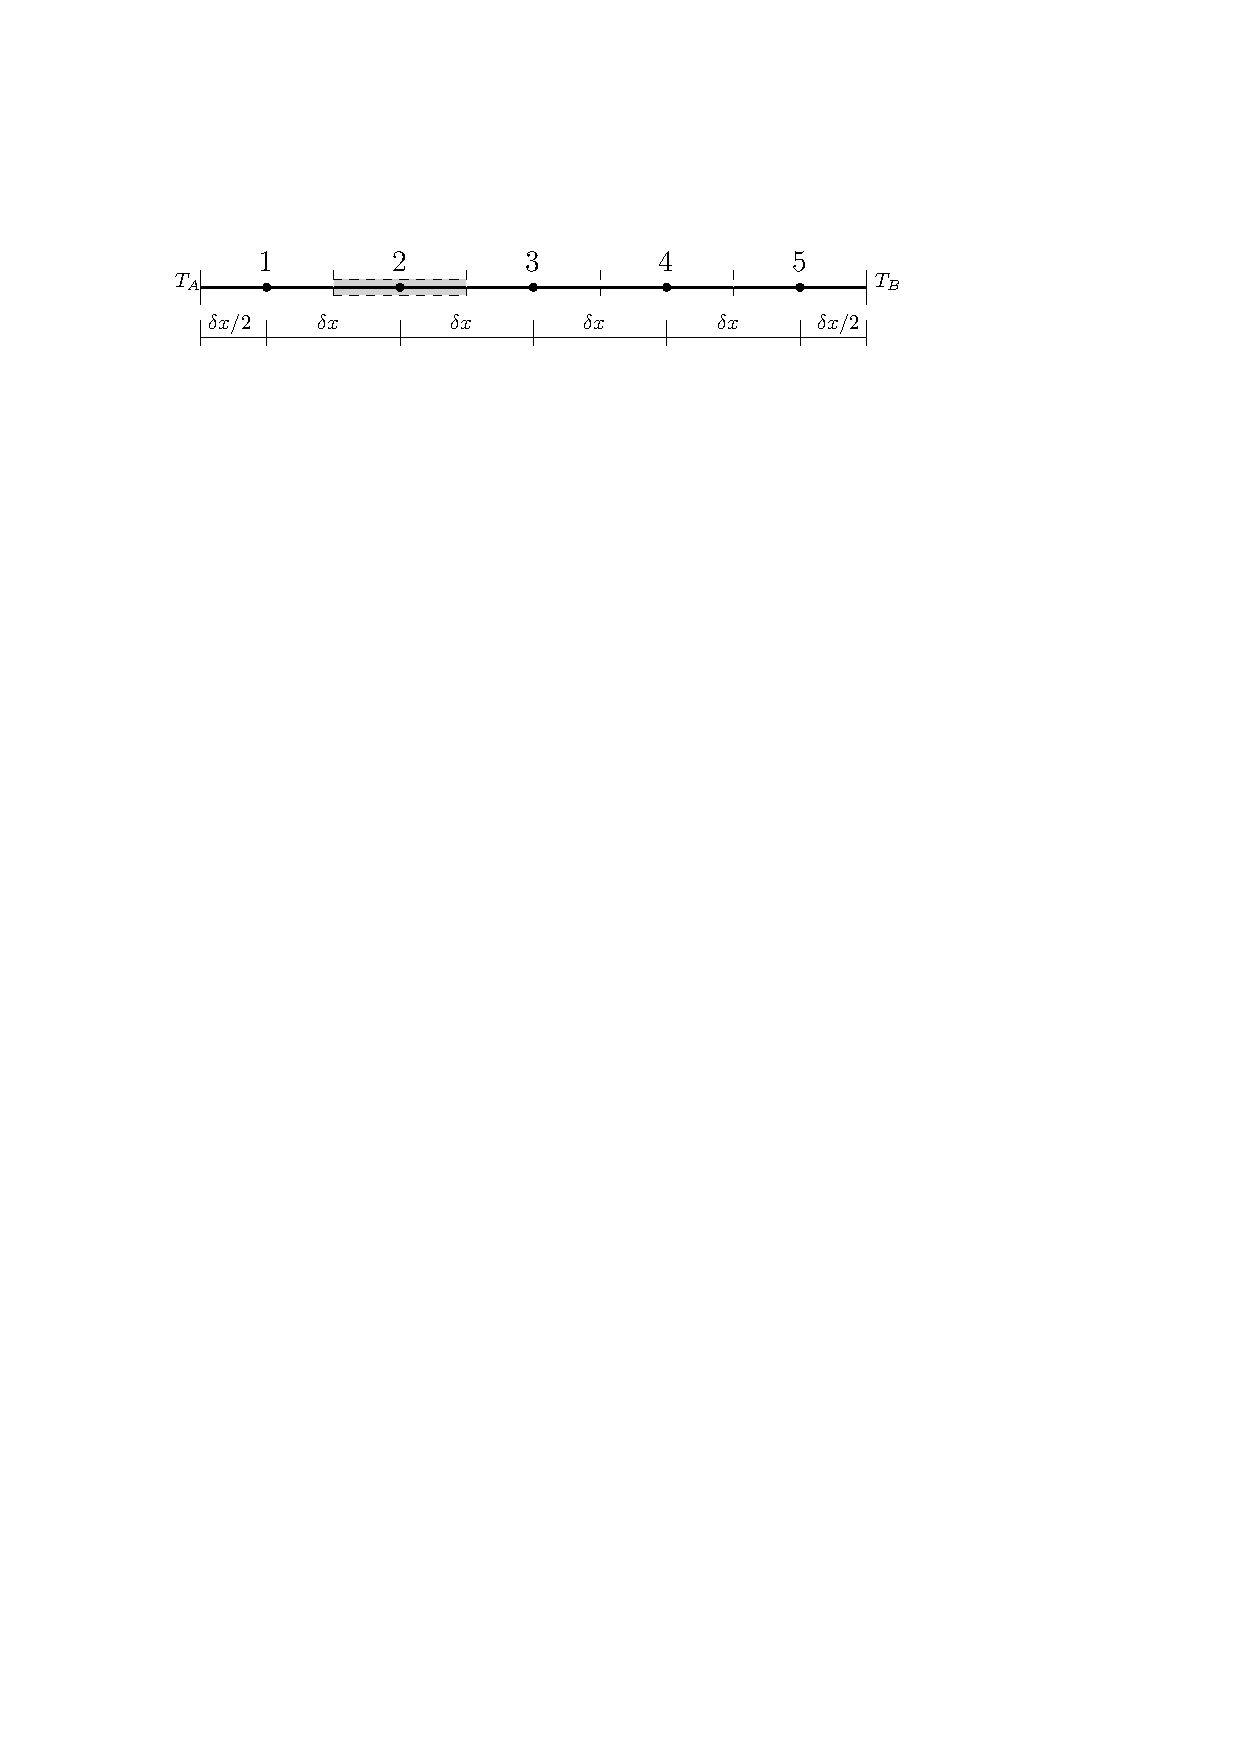
\includegraphics{FVmEx1Mesh.pdf}
  \caption{一维金属棒网格系统}
  \label{FgFV_ex1_grid}
\end{figure}

对节点2,3和4,
\begin{equation}
  \left(
    \frac{k}{\delta x_{PE}}A_{e}
    +
    \frac{k}{\delta x_{WP}}A_{w}
  \right)
  T_{P}
  =
  \left(
    \frac{k}{\delta x_{WP}}A_{w}
  \right)
  T_{W}
  +
  \left(
    \frac{k}{\delta x_{PE}}A_{e}
  \right)
  T_{E}
\end{equation}
由于导热系数,截面面积和网格间距为常数,因此上式可以写出:
\begin{equation}
  a_{P}T_{P} = a_{W}T_{W} + a_{E}T_{E}
\end{equation}
其中
\begin{table}[H]
  \begin{center}
  %\caption{雅可比迭代结果}
  \label{TbFV_diffusion_coefficient_ex1_n234}
  \begin{tabular}{|c|c|c|}
    \hline
    $a_{W}$ & $a_{E}$ & $a_{P}$
    \\
    \hline
    \makecell*[c]{
    $\displaystyle \frac{k}{\delta x}A$
  }
            &
    $\displaystyle \frac{k}{\delta x}A$
            &
    $a_{W} + a_{E}$
    \\
    \hline
  \end{tabular}
  \end{center}
\end{table}
对节点1,将式\eqref{EqFV_1dsd_ex1_gov}在包围节点1的控制体上
积分,可得
\begin{equation}
kA
\left(
  \frac{T_{E}-T_{P}}{\delta x}
\right)
-
kA
\left(
  \frac{T_{P}-T_{A}}{\delta x/2}
\right)
=
0
\end{equation}
对上式进行移项,可得
\begin{equation}
  \left(
    \frac{k}{\delta x}A
    +
    \frac{2k}{\delta x}A
  \right)
  T_{P}
  =
  0\cdot T_{W}
  +
  \left(
    \frac{k}{\delta x}A
  \right)
  T_{E}
  +
  \left(
    \frac{2k}{\delta x}A
  \right)
  T_{A}
\end{equation}
写成离散形式:
\begin{equation}
  a_{P}T_{P}
  =
  a_{W}T_{W}
  +
  a_{E}T_{E}
  +
  S_{u}
\end{equation}
其中
\begin{table}[H]
  \begin{center}
  %\caption{雅可比迭代结果}
  \label{TbFV_diffusion_coefficient_ex1_n1}
  \begin{tabular}{|c|c|c|c|c|}
    \hline
    $a_{W}$ & $a_{E}$ & $a_{P}$ & $S_{p}$ & $S_{u}$
    \\
    \hline
    0
            &
    \makecell*[c]{
    $\displaystyle \frac{kA}{\delta x}$
  }
            &
          $a_{W}+a_{E}-S_{p}$
            &
    \makecell*[c]{
    $\displaystyle -\frac{2kA}{\delta x}$
  }
  &
    \makecell*[c]{
      $\displaystyle \frac{2kA}{\delta x}T_{A}$
  }
    \\
    \hline
  \end{tabular}
  \end{center}
\end{table}


对节点5,将式\eqref{EqFV_1dsd_ex1_gov}在包围节点5的控制体上
积分,可得
\begin{equation}
kA
\left(
  \frac{T_{B}-T_{P}}{\delta x/2}
\right)
-
kA
\left(
  \frac{T_{P}-T_{W}}{\delta x}
\right)
=
0
\end{equation}
对上式进行移项,可得
\begin{equation}
  \left(
    \frac{k}{\delta x}A
    +
    \frac{2k}{\delta x}A
  \right)
  T_{P}
  =
  \left(
    \frac{k}{\delta x}A
  \right)
  T_{W}
  +
  0\cdot T_{E}
  +
  \left(
    \frac{2k}{\delta x}A
  \right)
  T_{B}
\end{equation}
写成离散形式:
\begin{equation}
  a_{P}T_{P}
  =
  a_{W}T_{W}
  +
  a_{E}T_{E}
  +
  S_{u}
\end{equation}
其中
\begin{table}[H]
  \begin{center}
  %\caption{雅可比迭代结果}
  \label{TbFV_diffusion_coefficient_ex1_n1}
  \begin{tabular}{|c|c|c|c|c|}
    \hline
    $a_{W}$ & $a_{E}$ & $a_{P}$ & $S_{p}$ & $S_{u}$
    \\
    \hline
    \makecell*[c]{
    $\displaystyle \frac{kA}{\delta x}$
  }
            &
    0
            &
          $a_{W}+a_{E}-S_{p}$
            &
    \makecell*[c]{
    $\displaystyle -\frac{2kA}{\delta x}$
  }
  &
    \makecell*[c]{
      $\displaystyle \frac{2kA}{\delta x}T_{B}$
  }
    \\
    \hline
  \end{tabular}
  \end{center}
\end{table}
将$kA/\delta x=100$,$T_{A}=100$和$T_{B}=500$代入5个节点的离散方程,可得
\begin{table}[H]
  \begin{center}
  %\caption{雅可比迭代结果}
  \label{TbFV_diffusion_coefficient_ex1_coeff}
  \begin{tabular}{|c|c|c|c|c|c|}
    \hline
    节点 & $a_{W}$ & $a_{E}$ & $S_{p}$ & $S_{u}$ & $a_{P}$ \\
    \hline
    1 & 0 & 100 & -200 & 20000 & 300  \\
    \hline
    2 & 100 & 100 & 0 & 0 & 200  \\
    \hline
    3 & 100 & 100 & 0 & 0 & 200 \\
    \hline
    4 & 100 & 100 & 0 & 0 & 200  \\
    \hline
    5 & 100 & 0 & -200 & 100000 & 300 \\ 
    \hline
  \end{tabular}
  \end{center}
\end{table}
最后形成的线性方程组为:
\begin{equation}
  \begin{bmatrix}
    300 & -100 & 0 & 0 & 0 \\
    -100 & 200 & -100 & 0 & 0 \\
    0 & -100 & 200 & -100 & 0 \\
    0 & 0 & -100 & 200 & -100  \\
    0 & 0 & 0 & -100 & 300 \\
  \end{bmatrix}
  \begin{bmatrix}
    T_{1} \\
    T_{2} \\
    T_{3} \\
    T_{4} \\
    T_{5} \\
  \end{bmatrix}
  =
  \begin{bmatrix}
    20000 \\
    0 \\
    0 \\
    0 \\
    100000 \\
  \end{bmatrix}
\end{equation}
通过上一章介绍的TDMA方法可以求得:
\begin{equation}
  \begin{bmatrix}
    T_{1} \\
    T_{2} \\
    T_{3} \\
    T_{4} \\
    T_{5} \\
  \end{bmatrix}
  =
  \begin{bmatrix}
    140 \\
    220 \\
    300 \\
    380 \\
    460 \\
  \end{bmatrix}
\end{equation}
该问题的解析解为$T=800x+100$。与解析解对比,可以看出数值解与解析解吻合程度很好。

\subsection{含源一维稳态热传导问题}
图\ref{FgFV_ex2}中显示的是一块厚度$L=2cm$的大平板,整块板内导热系数为常数
$k=0.5\mathrm{W/m\cdot K}$,板内存在均匀的内热源$q=1000\mathrm{kW/m^{3}}$。平板
$A$面和$B$面上的温度分别为$100^{\circ}\mathrm{C}$和$200^{\circ}\mathrm{C}$。假定
平板在$y$和$z$方向上大到只有$x$方向存在显著的温度梯度。试求稳态温度分布。

该问题的控制方程为:
\begin{equation}
\frac{\mathrm{d} }{\mathrm{d} x}
\left(
  k
  \frac{\mathrm{d} T}{\mathrm{d} x}
\right)
+
q
=
0
\end{equation}
网格系统继续采用图\ref{FgFV_ex1_grid}中所示的网格。在一个控制体上对控制方程积分
,
\begin{equation}
  \int_{\Delta V}\!
\frac{\mathrm{d} }{\mathrm{d} x}
\left(
  k
  \frac{\mathrm{d} T}{\mathrm{d} x}
\right)
\mathrm{d}V
+
  \int_{\Delta V}\!
  q
\mathrm{d}V
=
0
\end{equation}
上式的第一项处理方式与第一个例子中一样,第二项积分为$q\Delta V$。最终,上式可以
写成:
\begin{equation}
  \left[
    \left(
      kA\frac{\mathrm{d} T}{\mathrm{d} x}
    \right)_{e}
    -
    \left(
      kA\frac{\mathrm{d} T}{\mathrm{d} x}
    \right)_{w}
  \right]
  +
  q\Delta V
  =
  0
\end{equation}
\begin{equation}
  \left[
    k_{e}A
    \left(
      \frac{T_{E}-T_{P}}{\delta x}
    \right)_{e}
    -
    k_{w}A
    \left(
      \frac{T_{P}-T_{W}}{\delta x}
    \right)_{w}
  \right]
  +
  qA\delta x
  =
  0
\end{equation}
对上式移项,得
\begin{equation}
  \left(
    \frac{k_{e}A}{\delta x}
    +
    \frac{k_{w}A}{\delta x}
  \right)
  T_{P}
  =
  \left(
    \frac{k_{w}A}{\delta x}
  \right)
  T_{W}
  +
  \left(
    \frac{k_{e}A}{\delta x}
  \right)
  T_{E}
  +
  qA\delta x
\end{equation}
将上式写成离散方程通用形式:
\begin{equation}
  a_{P}T_{P} = a_{W}T_{W}+a_{E}T_{E}+S_{u}
  \label{EqFV_ex2_coeff}
\end{equation}
其中:
\begin{table}[H]
  \begin{center}
  %\caption{雅可比迭代结果}
  \label{TbFV_ex2_coef}
  \begin{tabular}{|c|c|c|c|c|}
    \hline
    $a_{W}$ & $a_{E}$ & $a_{P}$ & $S_{p}$ & $S_{u}$
    \\
    \hline
    \makecell*[c]{
    $\displaystyle \frac{kA}{\delta x}$
  }
            &
    $\displaystyle \frac{kA}{\delta x}$
            &
    $a_{W} + a_{E} - S_{P}$
            &
            0
            &
            $qA\delta x$
    \\
    \hline
  \end{tabular}
  \end{center}
\end{table}
式\eqref{EqFV_ex2_coeff}对网格中内部节点2,3,4都是通用的。

对边界节点1,控制方程在包含节点1的控制体内积分,
\begin{equation}
  \left[
    \left(
      kA\frac{\mathrm{d} T}{\mathrm{d} x}
    \right)_{e}
    -
    \left(
      kA\frac{\mathrm{d} T}{\mathrm{d} x}
    \right)_{w}
  \right]
  +
  q\Delta V
  =
  0
\end{equation}
\begin{equation}
  \left[
    k_{e}A
    \left(
      \frac{T_{E}-T_{P}}{\delta x}
    \right)
    -
    k_{A}A
    \left(
      \frac{T_{P}-T_{A}}{\delta x/2}
    \right)
  \right]
  +
  qA\delta x
  =
  0
\end{equation}
对上式移项,得
\begin{equation}
  \left(
    \frac{k_{e}A}{\delta x}
    +
    \frac{2k_{A}A}{\delta x}
  \right)
  T_{P}
  =
  0\cdot
  T_{W}
  +
  \left(
    \frac{k_{e}A}{\delta x}
  \right)
  T_{E}
  +
  \frac{2k_{A}A}{\delta x}T_{A}
  +
  qA\delta x
\end{equation}
将上式写成离散方程通用形式,且将导热系数为常数$k$代入:
\begin{equation}
  a_{P}T_{P} = a_{W}T_{W}+a_{E}T_{E}+S_{u}
  \label{EqFV_ex2_coeff}
\end{equation}
其中:
\begin{table}[H]
  \begin{center}
  %\caption{雅可比迭代结果}
  \label{TbFV_ex2_coef}
  \begin{tabular}{|c|c|c|c|c|}
    \hline
    $a_{W}$ & $a_{E}$ & $a_{P}$ & $S_{p}$ & $S_{u}$
    \\
    \hline
    0
            &
    \makecell*[c]{
    $\displaystyle \frac{kA}{\delta x}$
  }
            &
    $a_{W} + a_{E} - S_{P}$
            &
           $\displaystyle -\frac{2kA}{\delta x} $
            &
            $\displaystyle qA\delta x+\frac{2kA}{\delta x}T_{A}$
    \\
    \hline
  \end{tabular}
  \end{center}
\end{table}

对边界节点5,控制方程在包含节点5的控制体内积分,
\begin{equation}
  \left[
    \left(
      kA\frac{\mathrm{d} T}{\mathrm{d} x}
    \right)_{e}
    -
    \left(
      kA\frac{\mathrm{d} T}{\mathrm{d} x}
    \right)_{w}
  \right]
  +
  q\Delta V
  =
  0
\end{equation}
\begin{equation}
  \left[
    k_{B}A
    \left(
      \frac{T_{B}-T_{P}}{\delta x/2}
    \right)
    -
    k_{w}A
    \left(
      \frac{T_{P}-T_{W}}{\delta x}
    \right)
  \right]
  +
  qA\delta x
  =
  0
\end{equation}
对上式移项,得
\begin{equation}
  \left(
    \frac{k_{w}A}{\delta x}
    +
    \frac{2k_{B}A}{\delta x}
  \right)
  T_{P}
  =
  \left(
    \frac{k_{w}A}{\delta x}
  \right)
  T_{W}
  +
  0\cdot
  T_{E}
  +
  \frac{2k_{B}A}{\delta x}T_{B}
  +
  qA\delta x
\end{equation}
将上式写成离散方程通用形式,且将导热系数为常数$k$代入:
\begin{equation}
  a_{P}T_{P} = a_{W}T_{W}+a_{E}T_{E}+S_{u}
  \label{EqFV_ex2_coeff}
\end{equation}
其中:
\begin{table}[H]
  \begin{center}
  %\caption{雅可比迭代结果}
  \label{TbFV_ex2_coef}
  \begin{tabular}{|c|c|c|c|c|}
    \hline
    $a_{W}$ & $a_{E}$ & $a_{P}$ & $S_{p}$ & $S_{u}$
    \\
    \hline
    \makecell*[c]{
    $\displaystyle \frac{kA}{\delta x}$
  }
            &
            0
            &
    $a_{W} + a_{E} - S_{P}$
            &
           $\displaystyle -\frac{2kA}{\delta x} $
            &
            $\displaystyle qA\delta x+\frac{2kA}{\delta x}T_{B}$
    \\
    \hline
  \end{tabular}
  \end{center}
\end{table}
将$A=1$,$k=0.5\mathrm{W/m\cdot K}$,$q=1000\mathrm{kW/m^{3}}$和$\delta
x=0.004\mathrm{m}$代入各节点离散方程,可以得出各离散方程中所有系数的值,如表所示
。
最终形成的线性方程组为
\begin{equation}
  \begin{bmatrix}
    375 & -125 & 0 & 0 & 0 \\
    -125 & 250 & -125 & 0 & 0  \\
    0 & -125 & 250 & -125 & 0   \\
    0 & 0 & -125 & 250 & -125  \\
    0 & 0 & 0 & -125 & 375 \\
  \end{bmatrix}
  \begin{bmatrix}
    T_{1} \\
    T_{2} \\
    T_{3} \\
    T_{4} \\
    T_{5} \\
  \end{bmatrix}
  =
  \begin{bmatrix}
    29000 \\
    4000 \\
    4000 \\
    4000 \\
    54000 \\
  \end{bmatrix}
\end{equation}
最终解得,
\begin{equation}
  \begin{bmatrix}
    T_{1} \\
    T_{2} \\
    T_{3} \\
    T_{4} \\
    T_{5} \\
  \end{bmatrix}
=
  \begin{bmatrix}
    150 \\
    218 \\
    254 \\
    258 \\
    230 \\
  \end{bmatrix}
\end{equation}

这个问题的解析解可以通过对控制方程进行两次积分,然后带入边界条件后得出,
\begin{equation}
  T 
  =
  \left[
    \frac{T_{B}-T_{A}}{L}
    +
    \frac{q}{2k}(L-x)
  \right]x
  +
  T_{A}
\end{equation}
数值解与解析解的详细对比见表\ref{TbFV_ex2_compare},可以看出数值解与解析解的误差
很小,最大相对误差不超过百分之三。
\begin{table}[H]
  \begin{center}
  \caption{数值解与解析解的对比数据}
  \label{TbFV_ex2_compare}
  \begin{tabular}{|c|c|c|c|c|c|}
    \hline
    节点编号 & 1 & 2 & 3 & 4 & 5 \\
    \hline
    $x(\mathrm{m})$ & 0.002 & 0.006 & 0.01 & 0.014 & 0.018 \\
    \hline
    $T_{FVM}(^{\circ}\mathrm{C})$ & 150 & 218 & 254 & 258 & 230 \\
    \hline
    $T_{exact}(^{\circ}\mathrm{C})$ & 146 & 214 & 250 & 254 & 226 \\
    \hline
    相对误差(\%) & 2.73 & 1.86 & 1.60 & 1.57 & 1.76 \\
    \hline
  \end{tabular}
  \end{center}
\end{table}

\subsection{一维金属杆对流散热问题}

\begin{equation}
  \frac{\mathrm{d}}{\mathrm{d}x}
  \left(
    kA\frac{\mathrm{d}T}{\mathrm{d}x}
  \right)
  -
  hP(T-T_{\infty})
  =
  0
\end{equation}
其中,$h$为对流换热系数,$P$为金属杆截面的周长,$k$为杆的导热系数,$T_{\infty}$
为杆周围流体的温度。该问题的解析解为
\begin{equation}
  \frac{T-T_{\infty}}{T_{B}-T_{\infty}}
  =
  \frac{\cosh{[n(L-x)]}}{\cosh{(nL)}}
\end{equation}
其中,$n^{2}=hP/(kA)=25/{\mathrm{m^{2}}}$

\begin{equation}
  \frac{\mathrm{d}}{\mathrm{d}x}
  \left(
  \frac{\mathrm{d}T}{\mathrm{d}x}
  \right)
  -
  n^{2}(T-T_{\infty})
  =
  0
\end{equation}

\begin{equation}
  \int_{\Delta V}\!
  \frac{\mathrm{d}}{\mathrm{d}x}
  \left(
  \frac{\mathrm{d}T}{\mathrm{d}x}
  \right)
  \mathrm{d}V
  -
  \int_{\Delta V}\!
  n^{2}(T-T_{\infty})
  \mathrm{d}V
  =
  0
\end{equation}

\begin{equation}
  \left[
    \left(
    A
      \frac{\mathrm{d}T}{\mathrm{d}x}
    \right)_{e}
    -
    \left(
    A
      \frac{\mathrm{d}T}{\mathrm{d}x}
    \right)_{w}
  \right]
  -
  n^{2}(T_{P}-T_{\infty})A\delta x
  =
  0
\end{equation}

\begin{equation}
  \left[
    \left(
      \frac{T_{E}-T_{P}}{\delta x}
    \right)
    -
    \left(
      \frac{T_{P}-T_{W}}{\delta x}
    \right)
  \right]
  -
  n^{2}(T_{P}-T_{\infty})\delta x
  =
  0
\end{equation}

\begin{equation}
  \left(
    \frac{1}{\delta x}
    +
    \frac{1}{\delta x}
  \right)T_{P}
  =
  \left(
    \frac{1}{\delta x}
  \right)T_{W}
  +
  \left(
    \frac{1}{\delta x}
  \right)T_{E}
  +
  n^{2}\delta xT_{\infty}
  -
  n^{2}\delta xT_{P}
\end{equation}

\begin{equation}
  a_{P}T_{P}
  =
  a_{W}T_{W}
  +
  a_{E}T_{E}
  +
  S_{u}
\end{equation}

\begin{table}[H]
  \begin{center}
  \label{TbFV_ex3_coeff}
  \begin{tabular}{|c|c|c|c|c|}
    \hline
    $a_{W}$ & $a_{E}$ & $a_{P}$ & $S_{p}$ & $S_{u}$
    \\
    \hline
    \makecell*[c]{
    $\displaystyle \frac{1}{\delta x}$
  }
            &
    $\displaystyle \frac{1}{\delta x}$
            &
          $a_{W}+a_{E}-S_{p}$
            &
            $-n^{2}\delta x$
  &
  $n^{2}\delta xT_{\infty}$
    \\
    \hline
  \end{tabular}
  \end{center}
\end{table}


\begin{equation}
  \left[
    \left(
      \frac{T_{E}-T_{P}}{\delta x}
    \right)
    -
    \left(
      \frac{T_{P}-T_{B}}{\delta x/2}
    \right)
  \right]
  -
  n^{2}(T_{P}-T_{\infty})\delta x
  =
  0
\end{equation}

\begin{table}[H]
  \begin{center}
  \label{TbFV_ex3_coeff}
  \begin{tabular}{|c|c|c|c|c|}
    \hline
    $a_{W}$ & $a_{E}$ & $a_{P}$ & $S_{p}$ & $S_{u}$
    \\
    \hline
    0
            &
    \makecell*[c]{
    $\displaystyle \frac{1}{\delta x}$
  }
            &
          $a_{W}+a_{E}-S_{p}$
            &
            $\displaystyle -n^{2}\delta x - \frac{1}{\delta x}$
  &
  $\displaystyle n^{2}\delta xT_{\infty}+\frac{2}{\delta x}T_{B}$
    \\
    \hline
  \end{tabular}
  \end{center}
\end{table}


\begin{equation}
  \left[
    0
    -
    \left(
      \frac{T_{P}-T_{W}}{\delta x}
    \right)
  \right]
  -
  n^{2}(T_{P}-T_{\infty})\delta x
  =
  0
\end{equation}

\begin{table}[H]
  \begin{center}
  \label{TbFV_ex3_coeff}
  \begin{tabular}{|c|c|c|c|c|}
    \hline
    $a_{W}$ & $a_{E}$ & $a_{P}$ & $S_{p}$ & $S_{u}$
    \\
    \hline
    \makecell*[c]{
    $\displaystyle \frac{1}{\delta x}$
  }
            &
    0
            &
          $a_{W}+a_{E}-S_{p}$
            &
            $-n^{2}\delta x$
  &
  $n^{2}\delta xT_{\infty}$
    \\
    \hline
  \end{tabular}
  \end{center}
\end{table}

\begin{equation}
  \begin{bmatrix}
    20 & -5 & 0 & 0 & 0 \\
    -5 & 15 & -5 & 0 & 0 \\
    0 & -5 & 15 & -5 & 0  \\
    0 & 0 & -5 & 15 & -5   \\
    0 & 0 & 0 & -5 & 10 \\
  \end{bmatrix}
  \begin{bmatrix}
    T_{1} \\
    T_{2} \\
    T_{3} \\
    T_{4} \\
    T_{5} \\
  \end{bmatrix}
  =
  \begin{bmatrix}
    1100 \\
    100 \\ 
    100 \\ 
    100 \\ 
    100 \\ 
  \end{bmatrix}
\end{equation}
\begin{equation}
  \begin{bmatrix}
    T_{1} \\
    T_{2} \\
    T_{3} \\
    T_{4} \\
    T_{5} \\
  \end{bmatrix}
  =
  \begin{bmatrix}
    64.22 \\
    36.91 \\ 
    26.50 \\ 
    22.60 \\ 
    21.30 \\ 
  \end{bmatrix}
\end{equation}

\begin{table}[H]
  \begin{center}
  \caption{例三数值解与解析解的对比数据}
  \label{TbFV_ex3_compare}
  \begin{tabular}{|c|c|c|c|c|c|}
    \hline
    节点 & $x(\mathrm{m})$ & $T_{FVM}$ & $T_{exact}$ & 误差 & 相对误差(\%) \\
    \hline
    1 & 0.1 & 64.22 & 68.52 & 4.30 & 6.27 \\
    \hline
    2 & 0.3 & 36.91 & 37.86 & 0.95 & 2.51 \\
    \hline
    3 & 0.5 & 26.50 & 26.61 & 0.11 & 0.41 \\
    \hline
    4 & 0.7 & 22.60 & 22.53 & -0.07 & -0.31 \\
    \hline
    5 & 0.9 & 21.30 & 21.21 & -0.09 & -0.42 \\
    \hline
  \end{tabular}
  \end{center}
\end{table}

\subsection{二维扩散问题的有限体积法}
\begin{equation}
\frac{\partial }{\partial x}
\left(
\Gamma \frac{\partial \phi}{\partial x}
\right)
+
\frac{\partial }{\partial y}
\left(
\Gamma \frac{\partial \phi}{\partial y}
\right)
+
S_{\phi}
=
0
\end{equation}

\begin{equation}
  \int_{\Delta V}\!
\frac{\partial }{\partial x}
\left(
\Gamma \frac{\partial \phi}{\partial x}
\right)
\mathrm{d}x\mathrm{d}y
+
  \int_{\Delta V}\!
\frac{\partial }{\partial y}
\left(
\Gamma \frac{\partial \phi}{\partial y}
\right)
\mathrm{d}x\mathrm{d}y
+
  \int_{\Delta V}\!
S_{\phi}
\mathrm{d}V
=
0
\end{equation}
\begin{equation}
  \left[
    \Gamma_{e} A_{e}
    \left(
      \frac{\partial \phi}{\partial x}
    \right)_{e}
    -
    \Gamma_{w} A_{w}
    \left(
      \frac{\partial \phi}{\partial x}
    \right)_{w}
  \right]
  +
  \left[
    \Gamma_{n} A_{n}
    \left(
      \frac{\partial \phi}{\partial y}
    \right)_{n}
    -
    \Gamma_{s} A_{s}
    \left(
      \frac{\partial \phi}{\partial y}
    \right)_{s}
  \right]
  +
  \overline{S}\Delta V
  =
  0
\end{equation}
\begin{equation}
  \left.\frac{\partial \phi}{\partial x}\right|_{e}=\frac{\phi_{E}-\phi_{P}}{\delta x_{PE}} 
    \quad
  \left.\frac{\partial \phi}{\partial x}\right|_{w}=\frac{\phi_{P}-\phi_{W}}{\delta x_{WP}} 
    \quad
  \left.\frac{\partial \phi}{\partial y}\right|_{n}=\frac{\phi_{N}-\phi_{P}}{\delta y_{PN}} 
    \quad
  \left.\frac{\partial \phi}{\partial y}\right|_{s}=\frac{\phi_{P}-\phi_{S}}{\delta y_{SP}} 
\end{equation}

\begin{equation}
  \Gamma_{e}A_{e}
  \frac{\phi_{E}-\phi_{P}}{\delta x_{PE}} 
  -
  \Gamma_{w}A_{w}
  \frac{\phi_{P}-\phi_{W}}{\delta x_{WP}} 
  +
  \Gamma_{n}A_{n}
  \frac{\phi_{N}-\phi_{P}}{\delta y_{PN}} 
  -
  \Gamma_{s}A_{s}
  \frac{\phi_{P}-\phi_{S}}{\delta y_{SP}} 
  +
  \overline{S}\Delta V
  =
  0
\end{equation}

\begin{equation}
  \begin{aligned}
  \left(
    \frac{\Gamma_{w}A_{w}}{\delta x_{WP}}
    \right.
    +
   & \frac{\Gamma_{e}A_{e}}{\delta x_{PE}}
    +
    \frac{\Gamma_{s}A_{s}}{\delta y_{SP}}
    +
    \left.
    \frac{\Gamma_{n}A_{n}}{\delta y_{PN}}
    -
    S_{p}
  \right)
  \phi_{P}
  = \\
  &\left(
    \frac{\Gamma_{w}A_{w}}{\delta x_{WP}}
  \right)
  \phi_{W}
  +
  \left(
    \frac{\Gamma_{e}A_{e}}{\delta x_{PE}}
  \right)
  \phi_{E}
  +
  \left(
    \frac{\Gamma_{s}A_{s}}{\delta y_{SP}}
  \right)
  \phi_{S}
  +
  \left(
    \frac{\Gamma_{n}A_{n}}{\delta y_{PN}}
  \right)
  \phi_{N}
  +
  S_{u}
  \end{aligned}
\end{equation}
\begin{equation}
  a_{P}\phi_{P} 
  =
  a_{W}\phi_{W} 
  +
  a_{E}\phi_{E} 
  +
  a_{S}\phi_{S} 
  +
  a_{N}\phi_{N} 
  +
  S_{u}
\end{equation}

\begin{table}[H]
  \begin{center}
  %\caption{雅可比迭代结果}
  \label{TbFV_diffusion_coefficient_2d}
  \begin{tabular}{|c|c|c|c|c|}
    \hline
    $a_{W}$ & $a_{E}$ & $a_{S}$ & $a_{N}$ & $a_{P}$
    \\
    \hline
    \makecell*[c]{
      $\displaystyle \frac{\Gamma_{w}A_{w}}{\delta x_{WP}}$
  }
            &
      $\displaystyle \frac{\Gamma_{e}A_{e}}{\delta x_{PE}}$
            &
      $\displaystyle \frac{\Gamma_{s}A_{s}}{\delta y_{SP}}$
            &
            $\displaystyle \frac{\Gamma_{n}A_{n}}{\delta y_{PN}}$
            &
            $a_{W} + a_{E} + a_{S} + a_{N} - S_{P}$
    \\
    \hline
  \end{tabular}
  \end{center}
\end{table}


\section{稳态对流扩散方程的有限体积法}
\begin{equation}
  \frac{\mathrm{d} }{\mathrm{d} x}(\rho u\phi)
  =
  \frac{\mathrm{d} }{\mathrm{d} x}
  \left(
    \Gamma \frac{\mathrm{d} \phi}{\mathrm{d} x}
    \right)
\end{equation}
\begin{equation}
  \frac{\mathrm{d} (\rho u)}{\mathrm{d} x}
  =
  0
\end{equation}
\begin{equation}
  (\rho uA\phi)_{e}
  -
  (\rho uA\phi)_{w}
  =
  \left(
    \Gamma A\frac{\mathrm{d} \phi}{\mathrm{d} x}
  \right)_{e}
  -
  \left(
    \Gamma A\frac{\mathrm{d} \phi}{\mathrm{d} x}
  \right)_{w}
\end{equation}
\begin{equation}
  (\rho uA)_{e} 
  -
  (\rho uA)_{w}
  =
  0
\end{equation}
\begin{equation}
F = \rho u , \quad D = \frac{\Gamma}{\delta x}
\end{equation}
\begin{equation}
  F_{e}\phi_{e} - F_{w}\phi_{w}
  =
  D_{e}(\phi_{E}-\phi_{P})
  -
  D_{w}(\phi_{P}-\phi_{W})
\end{equation}
\begin{equation}
  F_{e} - F_{w} = 0
\end{equation}

\subsection{中心差分各式}
\begin{equation}
  \phi_{e} = (\phi_{P}+\phi_{E})/2
  \quad
  \phi_{w} = (\phi_{W}+\phi_{P})/2
\end{equation}

\begin{equation}
  \frac{F_{e}}{2}(\phi_{P}+\phi_{E})
 -
 \frac{F_{w}}{2}(\phi_{W}+\phi_{P})
  =
  D_{e}(\phi_{E}-\phi_{P})
  -
  D_{w}(\phi_{P}-\phi_{W})
\end{equation}
\begin{equation}
  \left[
    \left(
      D_{w} - \frac{F_{w}}{2}
    \right)
    +
    \left(
      D_{e} + \frac{F_{e}}{2}
    \right)
  \right]
  \phi_{P}
  =
    \left(
      D_{w} + \frac{F_{w}}{2}
    \right)
    \phi_{W}
    +
    \left(
      D_{e} - \frac{F_{e}}{2}
    \right)
    \phi_{E}
\end{equation}

\begin{equation}
  \left[
    \left(
      D_{w} + \frac{F_{w}}{2}
    \right)
    +
    \left(
      D_{e} - \frac{F_{e}}{2}
    \right)
    +
    (F_{e}- F_{w})
  \right]
  \phi_{P}
  =
    \left(
      D_{w} + \frac{F_{w}}{2}
    \right)
    \phi_{W}
    +
    \left(
      D_{e} - \frac{F_{e}}{2}
    \right)
    \phi_{E}
\end{equation}
\begin{equation}
  a_{P}\phi_{P}
  =
  a_{W}\phi_{W}
  +
  a_{E}\phi_{E}
\end{equation}

\begin{table}[H]
  \begin{center}
  %\caption{雅可比迭代结果}
  \label{TbFV_cd_cd_coefficient}
  \begin{tabular}{|c|c|c|}
    \hline
    $a_{W}$ & $a_{E}$ & $a_{P}$
    \\
    \hline
    \makecell*[c]{
      $\displaystyle D_{w}+\frac{F_{w}}{2}$
  }
            &
            $\displaystyle D_{e}-\frac{F_{e}}{2}$
            &
            $a_{W} + a_{E} + (F_{e} - F_{w})$
    \\
    \hline
  \end{tabular}
  \end{center}
\end{table}

\section{非稳态方程的有限体积法}

